\hfill \newline
\phantom{ } We built the circuit in figure[\ref{fig:cir}] with a resistor of $10\mathrm{k\Omega}$ and a capacitor of
$0.01\mathrm{\mu F}$. However, the actual resistance and capacitance we got are $R_1=10.1\mathrm{k\Omega}$ and $C_1=0.0183\mathrm{\mu F}$. Thus, $\tau_1 = R_1C_1 = 0.185\mathrm{\mu s}$. \newline
\phantom{ } We set the function generator to provide a square wave input with the period $T=4.00000000\mathrm{ms}$ and the voltage of $V_{pp}=5\mathrm{V}$ with offset $+2.5\mathrm{V}$, which generates a square wave of maximum voltage $5\mathrm{V}$ and minimum $0\mathrm{V}$.

\begin{figure}[!htbp]
	\centering
	\begin{framed}
	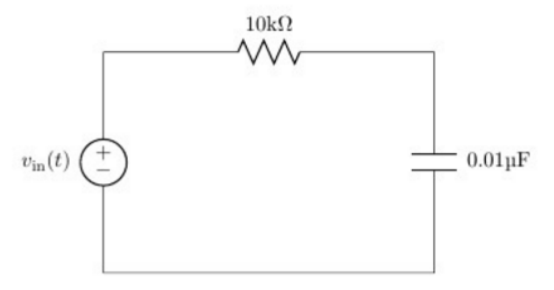
\includegraphics[width=\linewidth]{images/1_1.PNG}
	\caption{RC circuit for square wave input analysis}
		\end{framed}
	\label{fig:cir}
\end{figure}

We used channel 1 of the oscilloscope to verify the input and measured the output voltage of the capacitor by channel 2. Figure[\ref{fig:osc1}] is the screen output of two and half cycles.

\begin{figure}[!htbp]
	\centering
	\begin{framed}
	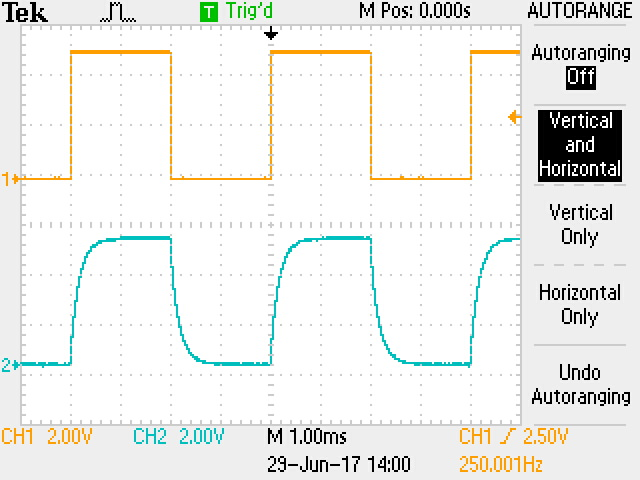
\includegraphics[width=0.95\linewidth]{images/1_2.JPG}
	\caption{The waveform of input and measure}
		\end{framed}
	\label{fig:osc1}
\end{figure}

\hfill \newline
\textbf{Analyze \#1:} \newline
\phantom{ } The oscilloscope did display the same waveform plotted in Prelab\#7. They are of the same shape, and both of their peaks and valleys reach the input waveform. Meanwhile, no obvious difference is found. \newline

Using the \textit{Cursor} menu, we recorded the period $T$, as well as the range of the output signal. Then we measured the time value of the $10\%$, $90\%$, and $50\%$ point of $V_{out}$. The results are shown in table[\ref{tab:mea}].

\begin{table}[!htbp]
	\centering
	\caption{Measurements of the output signal}
	\begin{tabular}{lrl}
		\toprule
		name & value & \\
		\midrule
		period & $4.000\mathrm{ms}$ & \\
		max voltage & $5.120\mathrm{V}$ & \\
		min voltage & $0.000\mathrm{V}$ & \\
		time of $10\% V_{out}$ (LH) & $20\mathrm{\mu s}$ & \\
		time of $90\% V_{out}$ (LH) & $480\mathrm{\mu s}$ & \\
		time of $50\% V_{out}$ (LH) & $124\mathrm{\mu s}$ & \\
		time of $10\% V_{out}$ (HL) & $12\mathrm{\mu s}$ & \\
		time of $90\% V_{out}$ (HL) & $394\mathrm{\mu s}$ & \\
		time of $50\% V_{out}$ (HL) & $106\mathrm{\mu s}$ & \\
		\bottomrule
	\end{tabular}
	\label{tab:mea}
\end{table}

\phantom{ } After calculating the rise time, fall time, and delay time of the RC circuit, we got table[\ref{tab:cal}]. Using the results we've calculated in prelab, both rise time and fall time are $2.2\tau$, and delay times are $0.69\tau$.

\begin{table}[!htbp]
	\centering
	\caption{Comparing actual values with theoretical values I}
	\begin{tabular}{lrrrl}
		\toprule
		name & actual value (calculated) & theoretical value & PE & \\
		\midrule
		rise time & $460\mathrm{\mu s}$ & ${407\mu s}$ & $13.0\%$ & \\
		fall time & $382\mathrm{\mu s}$ &  ${407\mu s}$ & $6.1\%$ & \\
		delay time (LH) & $124\mathrm{\mu s}$ & ${128\mu s}$ & $3.1\%$ & \\
		delay time (HL) & $106\mathrm{\mu s}$ &  ${128\mu s}$ & $17.2\%$ & \\
		\bottomrule
	\end{tabular}
	\label{tab:cal}
\end{table}

\hfill \newline
\textbf{Analysis \#2:} \newline
\phantom{ } There are a few reasons that can lead to the error. First, the $10\%$, $90\%$, and $50\%$ points we measured on the oscilloscope were not precise. We could not set the cursor the exactly the points. Second, their might be error with the capacitance measured by \textit{Digit Multimeter}. The capacitance may be lower than it is measured, for the reason that most actual values are lower than their theoretical value. Finally, the oscilloscope itself might interfere with the circuit, causing minor systematic error.

\begin{table}[!htbp]
	\centering
	\caption{Comparing actual values with theoretical values II}
	\begin{tabular}{lrrrl}
		\toprule
		name & actual value (measured) & theoretical value & PE & \\
		\midrule
		rise time & $348\mathrm{\mu s}$ & ${407\mu s}$ & $14.5\%$ & \\
		fall time & $369\mathrm{\mu s}$ &  ${407\mu s}$ & $9.3\%$ & \\
		delay time (LH) & $124\mathrm{\mu s}$ & ${128\mu s}$ & $3.1\%$ & \\
		delay time (HL) & $106\mathrm{\mu s}$ &  ${128\mu s}$ & $17.2\%$ & \\
		\bottomrule
	\end{tabular}
	\label{tab:dir}
\end{table}

\hfill \newline
\textbf{Analysis \#3:} \newline
\phantom{ } As is shown in table[\ref{tab:dir}], the automatically measured figures are all lower than the theoretical ones. The final two reasons of Analyze \#2 can also cause the error here. Compare those with quantities in table[\ref{tab:cal}], we can learn that the first reason mentioned in Analyze \#2 is not the major problem. Although we cannot make sure that the point we measured is precise, the oscilloscope's automatically measurement did not improve the PE result greatly.\newline